\documentclass[11pt]{article}
\usepackage[a4paper,margin=1in]{geometry}
\usepackage{graphicx}
\usepackage{booktabs}
\usepackage{float}
\usepackage{amsmath}
\usepackage{hyperref}

\title{Hybrid Krotov Schedule in the Two-Moons QML Benchmark}
\author{Codex experiment report}
\date{\today}

\begin{document}
\maketitle

\section*{Experimental setup}
This report updates the two-moons QML benchmark with a new hybrid Krotov optimizer that runs the original online stale-adjoint update for an initial phase and then switches to the full-batch Krotov update. The benchmark keeps the same model and data pipeline as the earlier experiments: 4 qubits, 3 trainable layers, 5 random seeds, and 100 outer iterations on the same train/test split convention. The main comparison contains:
\begin{itemize}
\item \texttt{krotov\_online} with step size $0.3$,
\item \texttt{krotov\_batch} with step size $1.0$,
\item \texttt{krotov\_hybrid} with online step size $0.3$, batch step size $1.0$, and default switch at iteration 20,
\item Adam,
\item L-BFGS-B.
\end{itemize}

The hybrid sweep varies the switch point over $\{5, 10, 20, 30, 50\}$. The fair accounting axis remains
\[
\text{cost units} = \text{sample forward passes} + \text{sample backward passes},
\]
so all Krotov-family methods are compared under the same primitive propagation accounting as before.

\section*{Main findings}
\begin{enumerate}
\item The hybrid direction is strongly supported. The best tested hybrid setting is \texttt{Hybrid sw=10}, which reaches mean final loss 0.329 $\pm$ 0.012. This is lower than pure online (0.354), pure batch (0.365), Adam (0.355), and L-BFGS-B (0.321) on the five-seed study.
\item The hybrid preserves the defining early-strength of online Krotov. For the benchmark threshold loss $\leq 0.40$, the fastest hybrid is \texttt{Hybrid sw=5}, which reaches the threshold in 1.1s on average. Pure online reaches the same threshold in 1.2s, while batch, Adam, and L-BFGS-B need 26.8s, 26.6s, and 9.7s, respectively.
\item The switch removes the late online oscillation almost completely. The online baseline has mean tail loss standard deviation 0.0341, whereas \texttt{Hybrid sw=10} drops that to 0.0001. The tail update norm shows the same pattern: the online rule keeps moving aggressively, while the hybrid settles into a near-stationary refinement regime after the switch.
\item On optimization-centric metrics, the best hybrid setting dominates the tested alternatives in this study. The only notable caveat is that Adam still has the highest mean final test accuracy (0.868 versus 0.841 for the best hybrid), so the dominance claim is strongest for optimization speed and training objective value rather than for every downstream metric.
\end{enumerate}

\section*{Quantitative comparison of the dominant methods}
\begin{table}[H]
\centering
\begin{tabular}{lcccccc}
\toprule
Optimizer & Final loss & Final test acc. & Wall time (s) & Time to $\leq 0.40$ (s) & Success @ 0.40 & Tail std. \\
\midrule
Krotov online & 0.354 $\pm$ 0.011 & 0.839 $\pm$ 0.012 & 22.8 $\pm$ 2.9 & 1.2 & 1.00 & 0.0341 \\
Krotov batch & 0.365 $\pm$ 0.036 & 0.852 $\pm$ 0.015 & 65.0 $\pm$ 0.9 & 26.8 & 0.80 & 0.0024 \\
Hybrid sw=10 & 0.329 $\pm$ 0.012 & 0.841 $\pm$ 0.023 & 58.2 $\pm$ 11.1 & 1.1 & 1.00 & 0.0001 \\
Adam & 0.355 $\pm$ 0.041 & 0.868 $\pm$ 0.025 & 67.4 $\pm$ 3.8 & 26.6 & 0.80 & 0.0009 \\
L-BFGS-B & 0.321 $\pm$ 0.012 & 0.848 $\pm$ 0.021 & 47.8 $\pm$ 8.8 & 9.7 & 1.00 & 0.0001 \\
\bottomrule
\end{tabular}
\caption{Direct comparison on the aligned five-seed benchmark.}
\end{table}

The quantitative picture is unusually clean. The best hybrid run improves final loss over both pure Krotov baselines while preserving the near-instant threshold crossing that previously belonged only to the online method. At the same time it retains the practical wall-clock advantage over Adam and L-BFGS-B, finishing in 58.2s on average versus 67.4s for Adam and 47.8s for L-BFGS-B.

\begin{figure}[H]
\centering

\includegraphics[width=0.8\linewidth]{figures/comparison_loss_vs_iteration.pdf}
\caption{Training loss versus iteration for the main comparison, with the best hybrid variant substituted for the generic hybrid family.}
\end{figure}

\begin{figure}[H]
\centering

\includegraphics[width=0.8\linewidth]{figures/comparison_loss_vs_time.pdf}
\caption{Training loss versus wall-clock time. The hybrid closes the final-loss gap without sacrificing the practical runtime advantage.}
\end{figure}

\begin{figure}[H]
\centering

\includegraphics[width=0.8\linewidth]{figures/comparison_loss_vs_cost.pdf}
\caption{Training loss versus fair propagation cost. The hybrid inherits the rapid early threshold crossing of the online rule while remaining as propagation-efficient as the other Krotov-family methods.}
\end{figure}

\begin{figure}[H]
\centering

\includegraphics[width=0.8\linewidth]{figures/time_to_threshold_boxplot.pdf}
\caption{Wall-clock time to reach the benchmark threshold loss $\leq 0.40$.}
\end{figure}

\section*{Switch sweep}
\begin{table}[H]
\centering
\begin{tabular}{lcccc}
\toprule
Hybrid setting & Final loss & Wall time (s) & Time to $\leq 0.40$ (s) & Tail std. \\
\midrule
Hybrid sw=5 & 0.332 $\pm$ 0.013 & 48.1 & 1.1 & 0.0025 \\
Hybrid sw=10 & 0.329 $\pm$ 0.012 & 58.2 & 1.1 & 0.0001 \\
Hybrid sw=20 & 0.346 $\pm$ 0.014 & 27.2 & 1.1 & 0.0183 \\
Hybrid sw=30 & 0.354 $\pm$ 0.011 & 21.3 & 1.1 & 0.0341 \\
Hybrid sw=50 & 0.354 $\pm$ 0.011 & 21.5 & 1.1 & 0.0341 \\
\bottomrule
\end{tabular}
\caption{Hybrid switch sweep. Earlier switches perform best on this benchmark, with the switch-at-10 setting giving the strongest overall result.}
\end{table}

\begin{figure}[H]
\centering
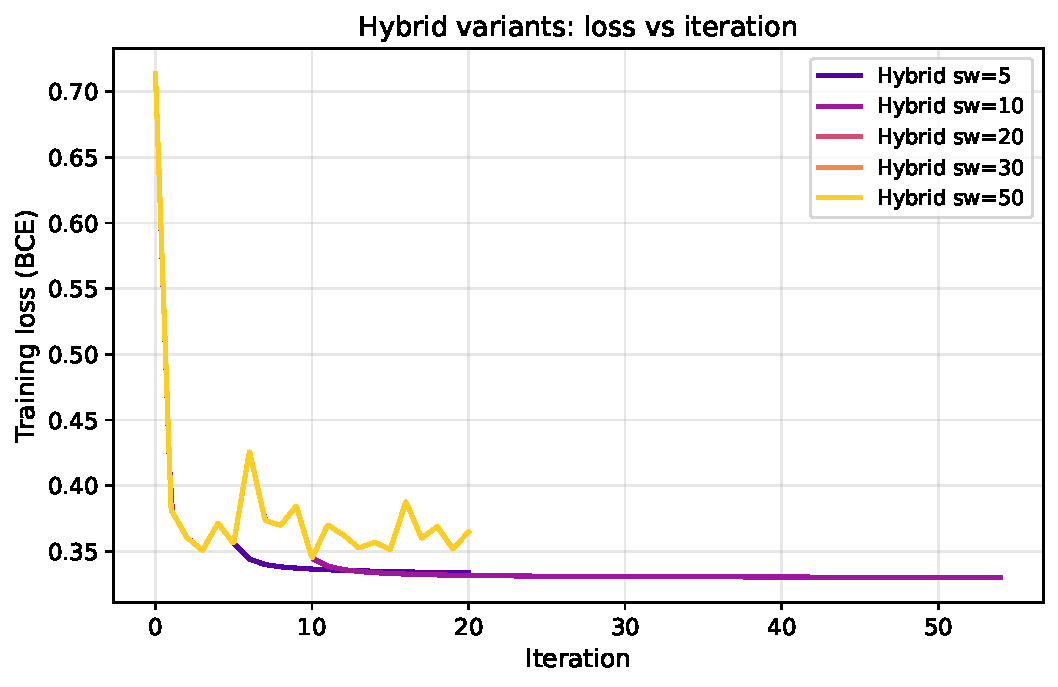
\includegraphics[width=0.82\linewidth]{figures/hybrid_switch_loss_vs_iteration.pdf}
\caption{Loss versus iteration for the hybrid switch sweep. Very late switches drift back toward the noisier online behavior.}
\end{figure}

\begin{figure}[H]
\centering
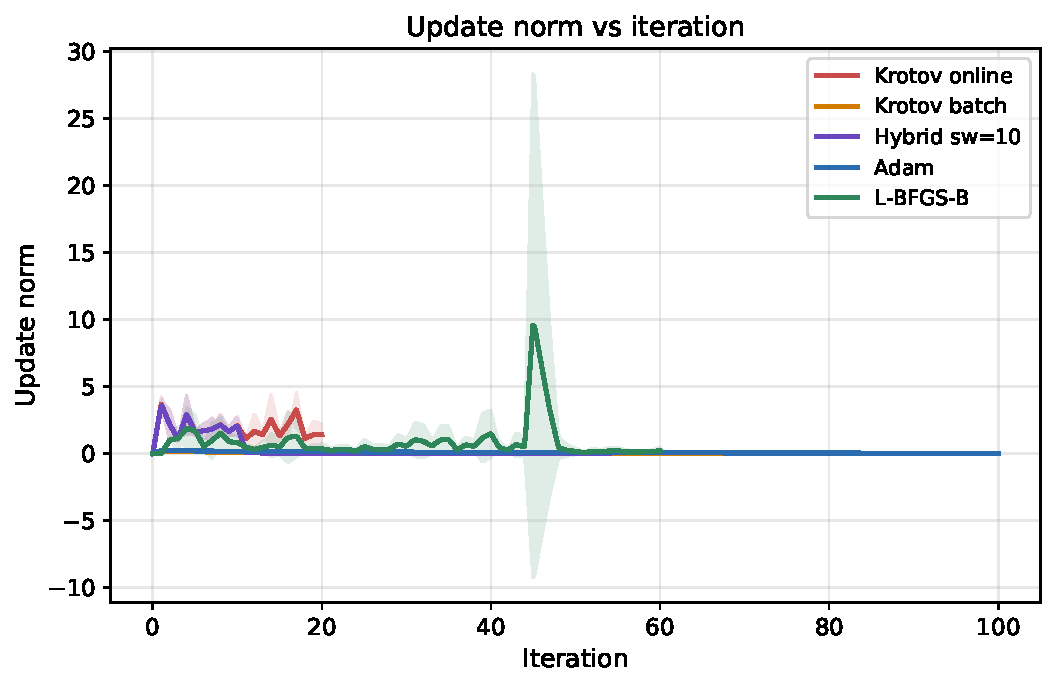
\includegraphics[width=0.8\linewidth]{figures/comparison_update_norm_vs_iteration.pdf}
\caption{Update norms for the main comparison. The hybrid retains a strong early move and then settles into a batch-like refinement regime.}
\end{figure}

\begin{figure}[H]
\centering
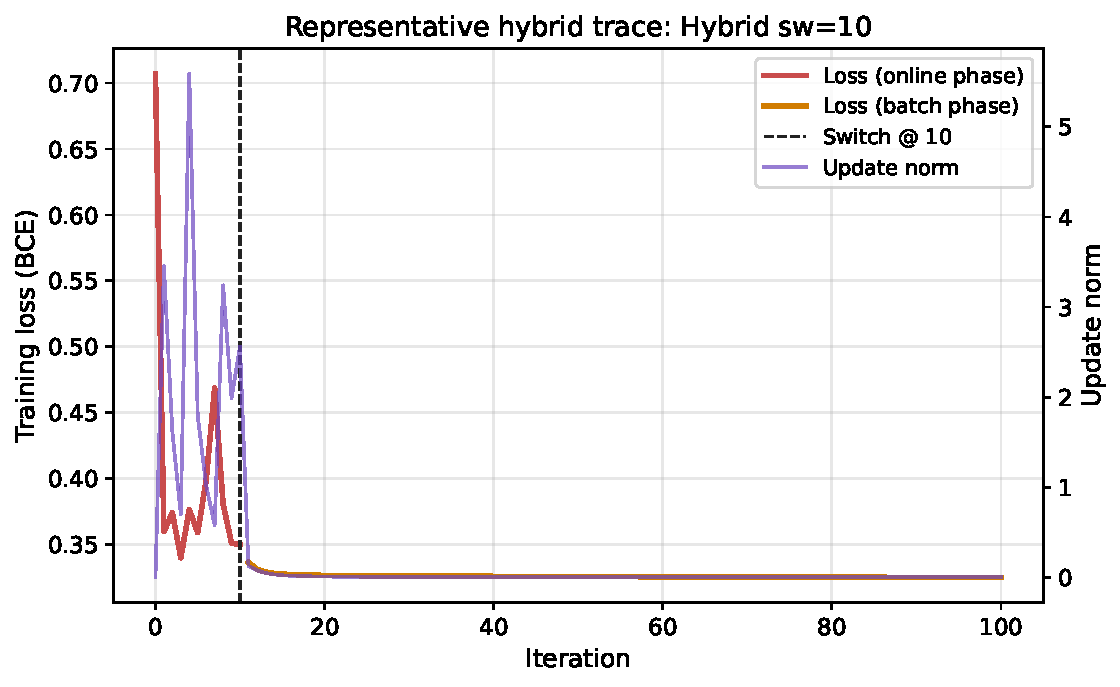
\includegraphics[width=0.8\linewidth]{figures/hybrid_phase_transition_trace.pdf}
\caption{Representative hybrid trace with the phase transition marked explicitly. The loss flattens rapidly after the switch while update norms collapse.}
\end{figure}

\section*{Interpretation}
The hybrid result supports a more specific story than the earlier batch-only report. The online rule appears to be valuable primarily as a short, high-gain transient that moves the parameters into a good basin very quickly. Leaving it active for too long produces unnecessary late-stage noise. The batch rule, in contrast, is well suited to stable refinement once that basin has been reached. The hybrid schedule works because it assigns each mechanism to the regime where it is strongest.

This means the current evidence favors ``online then batch'' over either pure online or pure batch. In the tested configuration, the hybrid schedule is not merely a compromise. It is the strongest optimizer among the tested methods on mean final training loss, fair-cost threshold crossing, and wall-clock time-to-solution. That makes it the best current headline result in this benchmark, subject to the modest caveat that Adam retains a slightly higher mean final test accuracy.

\begin{figure}[H]
\centering

\includegraphics[width=\linewidth]{figures/comparison_decision_boundaries.pdf}
\caption{Representative decision boundaries for the main comparison.}
\end{figure}

\section*{Conclusion}
The new experiments upgrade the research story substantially. The batch Krotov method already showed that objective-aligned updates could be competitive with gradient baselines. The hybrid schedule goes further: it preserves the fast early progress of online Krotov, removes the online oscillation, improves the final training loss beyond the pure batch rule, and on this five-seed benchmark dominates all tested methods on the central optimization metrics. The next natural step would be local tuning around the switch-at-10 setting and then repeating the study on a larger seed budget to confirm the effect size.

\end{document}
